\documentclass[oneside]{book}
\usepackage[utf8x]{inputenc}
\usepackage{amsmath}
\usepackage{amssymb}
\usepackage{amsfonts}
\usepackage{amsthm}
\usepackage{ucs}
\usepackage{cite}
\usepackage{newclude}
\usepackage{stmaryrd}
\usepackage[colorlinks]{hyperref}
\usepackage[titletoc,page]{appendix}
\usepackage[stable]{footmisc}
\usepackage{xifthen}
\usepackage{graphicx}
\usepackage{varioref}
\usepackage{syntax}
\usepackage{exercise}
\usepackage{xspace}
\usepackage{algorithm}
\usepackage[noend]{algpseudocode}

\newcommand*{\pfunc}{\xrightarrow{p}}
\newcommand*{\peq}{\simeq}
\newcommand*{\floor}[1]{\left\lfloor #1 \right\rfloor}
\newcommand*{\listOf}[1]{\left< #1 \right> }
\newcommand*{\coded}[1]{\ulcorner #1 \urcorner }
\newcommand*{\turingletter}[1]{\left< #1 \right> }
\newcommand*{\WHILE}{\ensuremath{\mathtt{WHILE}}\xspace}
\newcommand*{\FOR}{\ensuremath{\mathtt{FOR}}\xspace}
\newcommand*{\TM}{\ensuremath{\mathtt{TM}}\xspace}
\newcommand*{\NTM}{\ensuremath{\mathtt{NTM}}\xspace}
\newcommand*{\N}{\ensuremath{\mathbb{N}}\xspace}
\newcommand{\lepower}{\leq}
\newcommand{\gepower}{\geq}
\newcommand{\epower}{\equiv}
\newcommand{\abs}[1]{\left|#1\right|}
\newcommand{\TIME}[1][]{\ensuremath{\mathtt{TIME}\ifthenelse{\isempty{#1}}{}{_{#1}}}}
\newcommand{\NTIME}[1][]{\ensuremath{\mathtt{NTIME}\ifthenelse{\isempty{#1}}{}{_{#1}}}}
\newcommand{\SPACE}[1][]{\ensuremath{\mathtt{SPACE}\ifthenelse{\isempty{#1}}{}{_{#1}}}}
\newcommand{\NSPACE}[1][]{\ensuremath{\mathtt{NSPACE}\ifthenelse{\isempty{#1}}{}{_{#1}}}}
\newcommand{\LOGTIME}{\ensuremath{\mathtt{LOGTIME}}}
\newcommand{\LOGSPACE}{\ensuremath{\mathtt{LOGSPACE}}}
\newcommand{\PTIME}{\ensuremath{\mathtt{PTIME}}\xspace}
\newcommand{\NPTIME}{\ensuremath{\mathtt{NPTIME}}\xspace}
\newcommand{\PSPACE}{\ensuremath{\mathtt{PSPACE}}}
\newcommand{\EXPTIME}{\ensuremath{\mathtt{EXPTIME}}}
\newcommand{\EXPSPACE}{\ensuremath{\mathtt{EXPSPACE}}}
\mathchardef\mhyphen="2D
\newcommand{\set}[1]{\left\{ #1 \right\}}
\newcommand{\reducesTo}{\leq}

% Note Commands
\newcommand{\citationneeded}{{\em (citation needed) } }
\newcommand{\lineofthought}[1]{{\bf [#1] }}
\newcommand{\TODO}{\ensuremath{\left<\mathbf{TODO}\right> }}
\newcommand{\DONE}{}

% Disabled Note Commands
\newcommand{\timeestimation}[1]{}
%\newcommand{\citationneeded}{}
%\newcommand{\lineofthought}[1]{}
%\newcommand{\TODO}{}

\newcommand{\interpret}[2][]{\ensuremath{\left\llbracket #2 \right\rrbracket
	\ifthenelse{\isempty{#1}}{}{_{#1}}}}
\newcommand{\Input}[1][]{\ensuremath{I
	\ifthenelse{\isempty{#1}}{}{_{#1}}}}
\newcommand{\Output}[1][]{\ensuremath{O
	\ifthenelse{\isempty{#1}}{}{_{#1}}}}
\newcommand{\Compiler}[3][]{\ensuremath{compile_{#2\rightarrow #3}
	\ifthenelse{\isempty{#1}}{}{^{#1}}}}
\newcommand{\Interpreter}[2][]{\ensuremath{interpret_{#2}
	\ifthenelse{\isempty{#1}}{}{^{#1}}}}
\newcommand{\measuretime}[2][]{\ensuremath{T_#2
	\ifthenelse{\isempty{#1}}{}{^{#1}}}}
\newcommand{\measurespace}[2][]{\ensuremath{S_#2
	\ifthenelse{\isempty{#1}}{}{^{#1}}}}
\newtheorem{prop}{Proposition}
\newtheorem{theorem}{Theorem}
\newtheorem{corollary}{Corollary}
\newtheorem{thesis}{Thesis}
\theoremstyle{definition}
\newtheorem{defn}{Definition}
\newtheorem*{example}{Example}




\author{Aaron Karper}
\newcommand{\titletext}{A Programming Language Oriented Approach to Computability}
\title{\titletext}
\date{}
\begin{document}
\begin{titlepage}
  \let\footnotesize\small
  \let\footnoterule\relax
  \let \footnote \thanks
  
  \begin{center}%
	\vspace{10em}
  	{\huge{\textsc{\titletext}}\\}%
  	\vskip 5em%
	{\LARGE{Bachelorarbeit\\der Philosophisch-naturwissenschaftlichen
  	 Fakult\"at der Universit\"at Bern}\par}%
  	\vskip 12em%
  	{\Large{vorgelegt von}\par}%
  	\vskip 1.5em%
  	{\Large{Aaron Karper}\par}%
  	{\Large{2013}\par}%
  	\vskip 6em%
  	{\Large{Leiter der Arbeit:}\par}%
  	{\Large{Professor Dr. Thomas Strahm}\par}%
	{\Large{Institut f\"ur Informatik und angewandte Mathematik}\par}%
  \end{center}\par	
  \thanks
  \vfil\null
\end{titlepage}

\tableofcontents
\chapter{Introduction}
	Computability and complexity are in some way the basics of what computer
science is about. Where algorithmics might answer what the currently best known
solution to a problem is, computability theory says if a solution can exist and
complexity theory gives the problem (not the concrete algorithm!) a general
assessment of its difficulty, i.e. no algorithm can solve the problem faster 
than its inert complexity.

For this one needs an idea what a problem is, and when it is solvable. A 
problem can be understood as getting some kind of input data $x\in \Input[A]$ 
and needing to produce an output value $y\in \Output[A]$, in other words: 
computing a function $f:\Input[A] \rightarrow \Output[A]$\footnote{Equivalently, 
a problem can be characterized as deciding if $x\in^? B$.}.

A problem is then considered solvable, if there is in some way a solution to 
it, but what a solution looks like, divides the minds: 

\paragraph{Turing and his machines}
Turing's approach is a very mechanical one: A machine that has memory in the 
form of an arbitrarily large tape and is in a certain state. Depending on the 
tape's content at the current position and the current state, it can write to 
the tape, change its state and move one cell to the left or to the right.

\paragraph{Kleene composes functions}
Kleene held it intuitively computable that there are some simple functions 
such as the projections, the constant functions, and the successor are 
computable and that the composition of two computable functions is again 
computable. Finally every function can be coded and the codes can then be executed.

\paragraph{Markov rewrites strings}
Markov noted that executing an algorithm is basically nothing but rewriting a 
string (the memory) according to some predefined rules.

\paragraph{Programing languages}
While each of these approaches is interesting in their own right, they do not 
reflect the intuitions of a modern computer scientist, who already knows 
about programming languages and is closer to them then to building machines 
or even mathematical constructs.

Nearly all modern languages try to capture the full spectrum of solvable 
problems. For the sake of this text, a very simple language is considered, 
which consists of elements common in modern languages.

\lineofthought{
	I need to explain stuff I'll need in the chapter \ref{sec:WHILE}, e.g. 
	turing completeness (?), what a programming language is, ...
	
	\begin{itemize}
		\item Data and Language
		\item Representation of a program vs its semantics.
		\item Turing completeness
	\end{itemize}
}
\subsection{What is a programming language?} % (fold)
\label{sub:What is a programming language}
Before we can talk about computability in programming languages, we need to 
define, what a programming language is. 

\lineofthought{
	A language is a set of lists of characters (so called words). A programming 
	language also has a semantic function 
	$\interpret{.}: A\rightarrow (\ensuremath{\mathbb{N}} \rightarrow \ensuremath{\mathbb{N}})$.
}

% subsection What is a programming language (end)

	\section{The {\tt FOR} language}
\label{sec:FOR}
\begin{table}[htb]
	\begin{grammar}
		<expression> ::= 
							`nil' 
				\alt 	`cons' <expression> <expression>
				\alt 	`hd' <expression>
				\alt 	`tl' <expression>
				\alt 	<variable>

		<statement-list> ::= <statement> ;\alt <statement> ; <statement-list>

		<block> ::= `{' <statement-list> `}'

		<statement> ::=
							<variable> `:=' <expression>
				\alt	`if' <expression> <block> <else-block>
				\alt	`for' <variable> `in' <expression> <block>
			
				<else-block> ::= <empty> \alt `else' <block>
				
				<program> ::= <name> `read' <variable> <block> `write' <variable>
	\end{grammar}
	\caption{The \FOR syntax \label{tab:FOR-syntax}}
\end{table}

\subsection{The Elements} % (fold)
\label{sub:The Elements}
The \FOR language contains only very basic commands, but they can be combined
to implement a huge number of algorithms. As the data structure, we choose 
the humble {\tt cons} cell, that contains only a reference as the head and 
another as the tail.\footnote{An observant reader will notice that this
structure stems from the building of linked lists.}
.
\begin{figure}[htb]
	\begin{center}
		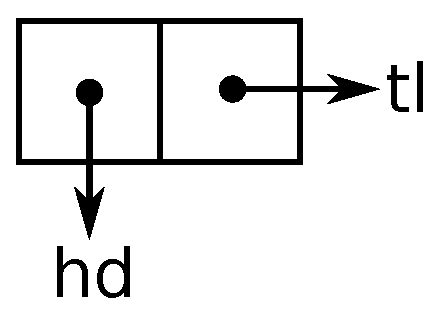
\includegraphics[height=3cm]{introduction/for/images/conscell}
	\end{center}
	\caption{The {\tt cons} cell}
\end{figure}

The expression {\tt cons e1 e2} constructs such a cell with the evaluation of
e1 in the head and the evaluation of e2 in the tail. The expression {\tt hd e1}
yields the head of the evaluation of e1 and {\tt tl e1} its tail. Since all our
current constructs need another expression, we also need a "bottom" to this
regress. We add {\tt nil} as an expression, which is distinct from any {\tt
cons e f}. We also want to refer to stored values, so an identifier (eg {\tt
X}) can also be an expression.

There are very few types of statements in \FOR, just three to be precise. The 
first is the {\em assignment} {\tt X := e}, which assigns the variable {\tt X}
the evaluation of {\tt e}. Later, when {\tt X} is used in an expression, it 
will reproduce this value. The second is the classic {\tt if} statement, that 
only executes its first block, if the expression does {\em not} return {\tt nil} 
and the else-block -- if any -- otherwise. Finally, there is the eponymous 
{\tt for} loop, that works as follows:

\begin{enumerate}
	\item On first entering the loop, the expression is evaluated and lets call 
		it $e$.
	\item If the evaluation is {\tt nil}, the loop is not evaluated anymore.
	\item Otherwise the block is evaluated with the value of the head of $e$.
	\item Then this procedure is run again with the tail of $e$.
\end{enumerate}

\subsection{\FOR computability}
The probably most important property of the \FOR language is that programs in 
it always terminate. The reason for this is, that upon entering the for loop, 
the number of repetitions is fixed as the length of the evaluated expression. 
Since we can't build an infinite expression in the finite time before the 
loop, the program terminates.

When experimenting with the language, one quickly finds, that many important 
functions are \FOR computable:

\begin{itemize}
	\item Constant functions.
	\item Addition.
	\item Multiplication -- as repeated addition.
	\item Exponentiation -- as repeated multiplication.
	\item Unary/binary conversion.
	\item Testing if a given number is prime.
	\item ...
\end{itemize}

As we can see, it is relatively simple to generate huge numbers using the 
\FOR language and then generate lists with that length.

\lineofthought{Thm: Algorithm $C$ with $T(C)\in O(f(n))$, $f(n) \in \FOR$, 
	then $\interpret{C}\in \FOR$}

At first glance it seems that any function can be computed this way, but 
sadly, that is not the case.

Intuitively the interpretation of a \FOR program should be computable. We can 
do it in an algorithmic way and so it is only reasonable to expect \FOR to be 
able to interpret itself. As we will see, that can not be the case:

\begin{theorem}
	There is no \FOR program $exec$ that takes $(program.input)$ as its 
	argument and returns $\interpret{program}(input)$.
\end{theorem}
\begin{proof}
Assume, there was a procedure in \FOR $exec$ that takes $(program.input)$ as 
its argument. Now the following procedure would surely be a \FOR program too:

\begin{verbatim}
inverse read X {
  result := [exec](X.X)
  if result {
    Y := FALSE
  } else {
    Y := TRUE
  }
} write Y
\end{verbatim}

We have 
\[ \interpret{inverse}(program) = \begin{cases}
		\mathtt{TRUE}, &\text{ if }\interpret{program}(program) = \mathtt{FALSE} \\
		\mathtt{FALSE}, &\text{ otherwise }
	\end{cases} \]

It outputs {\tt TRUE} iff the given program outputs {\tt FALSE}. What then 
is $\interpret{inverse}(inverse)$? Assume first that it is 
{\tt TRUE}, then by definition it is {\tt FALSE} -- and vice versa! So it 
neither returns {\tt TRUE} {\em nor} {\tt FALSE}. The only way that would 
work would be if it didn't return anything at all, but as we have seen, all 
\FOR programs terminate in finite time, so that can not be the case. 
Therefore {\tt inverse} can not be a \FOR program and by extension {\tt exec} 
is not a \FOR program. 
\footnote{This is the quitessential uncomputability 
	proof: A coding of the function is given that can be evaluated, but running 
  the program on itself leads to complications.}
\end{proof}

This is unfortunate, not only because we have seen that there are functions 
that are not \FOR computable, but that in general, any language that supports 
the building blocks of {\tt inverse} either doesn't support 
self-interpretation or it contains programs that will not halt.

As we try to capture {\em all} intuitively computable functions, it is not 
acceptable to leave self-interpretation out, so in the next chapter, we will 
explore a language that will contain non-halting programs.

\subsection{The \FOR in real programming languages}
It turns out, that while the {\tt for} keyword exists in most languages in 
one form or another, few acurately model the \FOR languages intention. 
Foremost most languages cheat around the property of \FOR loops always 
terminating: In C-like languages, the loop variable is not immutable and therefore
\begin{verbatim}
	for (int i = 0; i < 10; i++) {
	  // ...
	}
\end{verbatim}
might very well not terminate, if {\tt i} is decremented in the body. 
Iterator-based loops can be tricked by implementing an iterator that does not 
halt, i.e. produces a new value on any {\tt next}.

\subsection{The \FOR in mathematics and logic}
The \FOR computable functions match a category of functions known as 
primitive recursive. A function is primitive recursive, if it is either
\begin{enumerate}
	\item A successor function $S_i(x_1,\dots,x_n) = x_i+1$
	\item A projection function $P_i(x_1,\dots,x_n) = x_i$
	\item In the form of primitive recursion:
		\begin{equation*}
			f(n,x_1,\dots,x_n) = \begin{cases}
				g(x_1,\dots,x_n), &\text{ if }n=0\\
				h(f(n-1, x_1, \dots, x_n), x_1,\dots,x_n),&\text{ else}
			\end{cases}
		\end{equation*}
		Where $g$ and $h$ are primitive recursive.
\end{enumerate}
It is easy to see that \FOR can compute any primitive recursive function:
The successor function and the projections are trivial, for the primitive 
recursion, we have programs $\interpret{G}=g$ and $\interpret{H}=h$ by 
induction assumtion\citationneeded. 

\begin{verbatim}
F read NX {
  N := hd NX
  Xs := tl NX
  Repetitions := [unary](N)
  Result := [G](Xs)
  Counter := 0
  FOR I IN Repetitions {
    Result := [H](Result.Xs)
  }
} write Result
\end{verbatim}

The other direction is in the exercises \TODO.

	\section{The {\tt WHILE} Language\timeestimation{15h}}
\label{sec:WHILE}
In the last chapter we saw an example of a function that is not computable 
with a \FOR program\footnote{The semantic function of \FOR}. However with a 
simple addition to the language, we gain all we need for a language.

The new statement is called $\mathtt{while}\: e\: \{ block \}$, and it does what one would expect:

\begin{itemize}
	\item It takes an expression $e$ and a block $block$.
	\item If the evaluation of the expression yields {\tt nil}, it does nothing.
	\item Otherwise, it executes the block and repeats this procedure.
\end{itemize}

\begin{equation}
	\interpret{\mathtt{while}\: e\: block}(c) = \begin{cases}
		c, &\text{ if }\interpret{e}=Nil\\
		(\interpret{\mathtt{while}\: e\: block} \circ \interpret{block})(c), &\text{otherwise}
	\end{cases}
\end{equation}

This new statement does not necessarily terminate, in fact {\tt WHILE 
(nil.nil) \{\}} would never halt. This means, that the semantic function 
does not give a total function back -- for some inputs the interpretation of 
the source does not halt.

Looking back at the proof of the uncomputable function in \FOR called
$inverse$, that took a program and returned the boolean inverse of that
programs output when run with itself as input. We asked what
$\interpret{inverse}(inverse)$ would be. Since it can't be $TRUE$ nor
$FALSE$, it must be $\bot$. This can also be seen in that
$\interpret{eval}(inverse.inverse)$ is just an infinite recursion. 

Of course it could be that while this proof does not work, something else might
prevent us from implementing the {\tt eval} procedure. As we will see in
~\ref{sec:self}, that is not the case.

Part of this work is an implementation of the \WHILE programming language, which can be found at \url{https://github.com/zombiecalypse/Bachelor-Thesis/wiki}.


\chapter{Computability}
	\section{Language Transforms\timeestimation{25h}} % (fold)
\label{sec:transforms}
In this chapter, we'll discuss how we can use the notion of a data 
representation of a program to get a standard toolchain.
\subsection{Language Subsets} % (fold)
\label{sub:Language Subsets}
\begin{defn}
	Let {\tt A} and {\tt B} be two languages such that each valid {\tt B} 
	program is also a valid {\tt A} program. Further 
	$\forall b\in B\, \forall d\in Dat(B): \interpret[A]{b}(d) = \interpret[B]{b}(d)$

	Then $B$ is a language subset of $A$ (and conversely $A$ is a superset of
	$B$), writen $B \subset A$.
\end{defn}
\paragraph{{\tt C++}  and {\tt C} } % (fold)
\label{par:Cpp and C}
{\tt C++} was designed to be a object-oriented superset to the popular {\tt C}
programming language, so that the new {\tt C++} code could use legacy {\tt C}
code without modification. This notion was important to raise the acceptance of
{\tt C++} with programmers and eased switching.
% paragraph Cpp and C (end)
% subsection Language Subsets (end)
\subsection{Interpreter} % (fold)
\label{sub:Interpreter}
Today programmers and machines seldom speak the same language. Programming in 
machine language is difficult, error-prone and unportable to name only a few 
drawbacks. However it seems reasonable to expect to be able to execute ones 
code nonetheless. Typically, we want our computer to interpret what we mean 
in our high-level programming language. An {\em interpreter} is such a program.

\begin{defn}
	An {\em interpreter} of $A$ is a program 
	\[\interpret[P]{interp}: A \times \Input[A] \longrightarrow \Output[A] \]
	\[ \interpret[P]{interp}(a, d) = \interpret[A]{a}(d) \]
\end{defn}

\lineofthought{ A language $A$ that can interpret $B$ is at least as powerful as $B$ }

\lineofthought{Interpreter are easier to write, but have an interpretation overhead}
% subsection Interpreter (end)
\subsection{Compiler} % (fold)
\label{sub:Compiler}
\lineofthought{
	\begin{itemize}
		\item Simple definition: language transformer.
		\item 3 stages: frontend, independent middle and backend.
	\end{itemize}
}
\paragraph{How the {\tt gcc} is ported} % (fold)
\label{par:gcc}
When a new machine architecture is build, there is the problem that there is 
not yet any compiler for it. The naïve solution would be to write a complete 
compiler in the new machine language, but that would be very cumbersome and 
inefficient to do that for every new processor build.

There are two parts to the problem: on one hand, there is not any compiler, 
that outputs the new machine lanugage and on the other hand, there is no 
compiler that runs on the new machines.

For the first problem, we see that of the three stages of a modern compiler,
only the backend really depends on the output language. Often the backend has 
a general variant that can be parametrized for many architectures.
\footnote{For the whole process of writing a {\tt gcc} backend, see \cite{nilsson2000porting}}

The second problem is nowadays solved by cross-compiling -- when the language 
the compiler is executed in and the output language differ. Another approach 
was to have a minimal (non-optimizing) compiler or an interpreter to do the 
first translation.
% paragraph How the gcc is ported (end)
% subsection Compiler (end)
\subsection{Futamura Projections} % (fold)
\label{sub:Futamura}
\subsubsection{Specializer} % (fold)
\label{ssub:Specializer}
\subsubsection{Futamura Projections} % (fold)
\label{ssub:Futamura Projections}
The notion of a specializer as a transformer of source code has lead to some 
interesting observations: \lineofthought{ 
	\begin{itemize}
		\item An interpreter spec'ed with source is executable ($\rightarrow$ 
			py2exe) 
			\begin{equation*}
			  \begin{split}
					\interpret[P]{\interpret[P]{spec}(interp_A, src)}(d) 
						&= \interpret[P]{interp_A}(src,d)\\
						&= \interpret[A]{src}(d)
			  \end{split}
			\end{equation*}
		\item A compiler is a specialized specializer with the step above.
			\begin{equation*}
			  \begin{split}
					\interpret[P]{\interpret[P]{spec}(spec, interp_A}(src)
						&= \interpret[P]{spec}(interp_A, src)
			  \end{split}
			\end{equation*}
		\item Repeat to get a compiler generator.
	\end{itemize} 
	Use types to visualize (
	$\interpret[P]{spec}: Input_1 \rightarrow \coded{\left( Input_2 \rightarrow Output \right)}$)
}

\lineofthought{
	Exercise: interpreter for {\tt while} is given. Make a compiler.
}

% subsubsection Futamura Projections (end)
\paragraph{The PyPy project} % (fold)
\label{par:The PyPy project}
\begin{example}
	The {\tt PyPy} project is an attempt to implement the popular {\tt
	Python}\footnote{\url{http://python.org/}} itself in a subset of {\tt Python}
	(called {\tt RPython}). Since {\tt Python} is an interpreted language, it
	would seem that this approach would lead to very slow execution, but that is
	not the case: PyPy uses Just-In-Time (JIT) specialization and compilation
	techniques in part described in \cite{psycho}.

	While the approach described in \ref{ssub:Specializer} is understood to be 
	executed before the actual program is run, it is also possible to run it 
	in parallel to the actual computation: Now the specializer can use 
	statistical information on the values. For example, while it might not be 
	obvious from the source that a certain value is constant and therefore a 
	static specializer might fail to set in, but a dynamic specializer can 
	determine this and produce a specialized function to call.

	For a highly dynamic language like {\tt Python}, it can lead to a hundredfold 
	speedup for very repetitive arithmetics\footnote{\cite{psycho}}.
\end{example}

% paragraph The PyPy project (end)

% subsubsection Specializer (end)
% subsection Futamura (end)

	\section{Turing-Completeness of a Language}
\label{sec:Turing Completeness}
In the dawn of computer science there were serveral ideas what computable 
means. Does it mean, that a machine can compute it, as Turing suggested? Or 
should we define some functions that should be computable and how they can be
combined to discuss the computability of a problem?

As it turned out, it does not matter -- the problems that can be solved in 
each of them are the same. This was shown by proving that the different 
mechanisms can simulate each other. By extension, a new formulism only needs 
to be able to simulate any of the existing formalisms to be at least as 
powerful as any of them. Thus came the expression {\em Turing complete} to 
describe, that a certain formalism can build any Turing machine.

This chapter is build as exercises, because solving the problems gives a good 
impression, how one could go about proving other things to be turing complete.

\subsection{The Turing Machine}
The Turing Machine (\TM) is a formalism that focuses on a possible physical 
implementation of a computing machine, although far from what is used today. 
It features an potentially infinite amount of tape on which the machine 
operates. From this tape, the machine can read and write the current cell and 
move its read-write-head one cell to the left or the right. Finally, the 
machine has a finite number of ``states of mind", comparable to a finite 
state machine.

In order to formally analyse the \TM, we can code what such a machine would 
do in the following way:

\begin{defn}
	\label{def:tm}
	A Turing Machine is a % TODO
\end{defn}

\begin{example}
	Adding one to a binary number.
\end{example}

\subsection{\WHILE is Turing complete}
By definition \ref{def:power}, we would need a compiler from \TM to \WHILE, 
but by \ref{thm:power-interpreter}, an interpreter suffices. Implementing such an 
interpreter will be the following exercise.

\begin{Exercise}[title={Interpreter for \TM},label={exc:tm},difficulty=2]
	\Question Show that we can implement a dictionary datastructure in \WHILE. 
		Implement {\tt insert} and {\tt lookup}.
	\Question Show how you can code the transition function in your map.
	\Question Implement the tape
		\subQuestion Can you keep track of your position in a list with two stacks?
		\subQuestion Implement the left and right movement 
		$\interpret{{\tt left}},\interpret{{\tt right}} : Tape \rightarrow Tape$ . Note that the list is 
			only potentially infinite, so you might in actuality run into the current edge.
	\Question Plug the pieces together to implement an interpreter {\tt turing(TM)} for turing machines.
		\subQuestion How many nested {\tt while} loops do you need?
\end{Exercise}

\subsubsection{\TM  is \WHILE-complete}
It could now be, that \WHILE is more powerful than \TM, so that one can 
actually compute more with a \WHILE program than one could with Turing 
Machines alone.

\begin{Exercise}[title={Interpreter for \WHILE in \TM},difficulty=4]
	In this exercise, we will build up a language that can be expressed in \TM 
	and will finally include \WHILE. This is complex, but you might solve 
	many low level implementation problems of programming languages in the progress.
	\Question Show an $n$-taped \TM to the one taped (where $n$ is of course fixed at
		compilation time). A $n$-taped turing machine has $n$ tapes that can be 
		independently moved and writen.
	\Question Show that you can use ``functions":
		\subQuestion Show that you can copy one tape to the current position on a 
			second tape.
		\subQuestion Show that for all \TM's {\tt A} and {\tt B} exists a turing 
			machine {\tt A;B} such that $\interpret[\TM]{A;B}(x) \peq
			\interpret[\TM]{B}(\interpret[\TM]{A}(x))$, i.e. that you can execute
			\TM's one after another.
		\subQuestion Argue how this could be used to implement a function call.
	\Question Show that you can implement a {\tt while} construct
		\subQuestion Given a \TM $A$ that prints {\tt T} or {\tt F} on a tape and 
			another \TM $B$, construct a \TM {\tt if A \{B\}} that runs $A$ 
			and then $B$ only if the second tape shows $T$.
		\subQuestion Modify this so that $B$ gets executed as long as $A$ returns {\tt T}.
	\Question Implement the {\tt cons} datastructure on the tape of a turing 
	machine. Note that you can add another tape to ``take notes" by merit of the first question.
		\subQuestion Implement {\tt cons}. {\em Hint: Be literal about 
		expressions like {\tt cons (cons nil nil) (cons nil nil)}.} 
		\subQuestion Implement {\tt hd} and {\tt tl}.
	\Question Show that you can implement a map, that can be used to save the variables.
		\subQuestion Implement a list of pairs.
		\subQuestion Given a name on one tape, can you look up the pair in the 
			list of tuples on a second tape that contains this name as the first
			component?
		\subQuestion Implement changing the variables by striking out the old 
			pair and appending a new one.
	\Question Argue, how you could now interpret \WHILE.
\end{Exercise}

These two exercises show, that $\WHILE\epower\TM$. This is important, since 
when showing something to be \WHILE-complete, we don't need to implement the 
\WHILE, but can use \TM instead, which is much simpler.

\subsection{The Normal Form Theorem}
\begin{theorem}[Normal Form Theorem]
	Every \WHILE program can be transformed into a \WHILE program with exactly 
	one {\tt while} loop. That is, all the inner constructs are taken from \FOR.
\end{theorem}
\begin{proof}
	Lets call the language of \WHILE programs, that are in the normal form $\WHILE_1$.
	We have seen that we can transform $\WHILE \rightarrow \TM$ and 
	$\TM \rightarrow \WHILE_1$. If we chain these (informal) compilation processes to 
	get a compiler $\WHILE \rightarrow \WHILE_1$.
\end{proof}

\subsection{Church's Thesis}
As mentioned, when the notion of computability was first developed, there 
were competing formalisms, but as it turned out, they were all equally 
powerful. This lead Alonzo Church to conjegure, that what the human sees 
as intuitively computable, is adequately formalized by any of these 
competitors. This is known as Church's Thesis (or Church-Turing Thesis).

\begin{quote}
	The Turing Machine adequately models what we hold for intuitively computable.
\end{quote}

We saw that \WHILE too is a competitor, since it is equally powerful to any 
of the other formalisms. We could then formulate it as follows:

\begin{quote}
	There is no intuitive extension of \WHILE that is more powerful than \WHILE.
\end{quote}

For example, we could add procedure calls, but that would not make any 
functions computable that were not computable before.

The thesis can not be formally proven, since it connects the informal concept 
of ``intuitively computable" with the formal Turing Machines, however the 
evidence that no-one has since found a physical mechanism, that could be 
exploited to calculate more than a \TM gives a strong indication, that the 
Church-Turing Thesis is true.

\subsubsection{\dots or is it?}
There has been some work, what would happen, if you added certain 
functionalities to Turing Machines (and by extension to \WHILE). 

Turing himself analysed socalled oracle machines, which are basically Turing 
Machines, but can answer specific questions to an oracle on a different tape, 
that would answer if a specific predicate is true for the value of the tape.
The halting problem for Turing Machines is not solvable on a normal \TM, but 
we could add an oracle for it. This would be more powerful than \TM, but it 
is not intuitively clear how one could build such an oracle. Also, we would 
find, that the oracle machine could not solve its own halting problem -- for 
very much the same reason that the original \TM can't solve its own.

Another line of thought is that, when we talk about these formalisms, we 
don't really care if humans find it intuitively computable, but rather that 
we could actually build a machine that computes it. This gives us the 
physical Church-Turing thesis: It is not possible to build a computer that 
can not be simulated on a \TM.

This is a thesis, that {\em can} be put to the test. While \TM rely on 
classical mechanics, some thought has been put into quantum computing. The 
model that is used to build quantum computers (qubits) are however not 
stronger than \TM. Faster yes, but not really stronger.

On a larger scale, it is possible to construct a computing device that orbits 
around a rotating black hole. An observer falling into the black hole could 
then use the infinite computation time in subjectively finite time. It has 
however been noted, that falling into a black hole might not be a good 
idea\citationneeded.

\subsubsection{The structured program theorem}
\lineofthought{
	\begin{enumerate}
		\item run programs one after another ({\tt ;})
		\item run either this or that ({\tt if})
		\item run until predicate is false ({\tt while})
	\end{enumerate}
	$\Rightarrow$ Turing complete
}
\lineofthought{
	List some surprisingly turing complete things, e.g. cellular automata (Rule 110), 
	string rewriting, ...

	Churches thesis: There is no intuitive extension to {\tt  WHILE} that is 
	stronger than {\tt WHILE}.

	Approximations of results, ... also work (linear slow-down). 

	Note that when there are side effects, we might be interested that a program
	does {\em not} terminate (e.g. our OS).

	Common features of turing complete languages: They can use their own 
	description (recursion theorem), if there is a primrec subset $P$, then you 
	can describe all programs with $P$ and one ''loop`` of $A\setminus P$ 
	(normal form theorem)
}

\subsection{Properties of Turing complete languages}

\lineofthought{
	\begin{itemize}
		\item Recursion theorem (explain the construction of the $Y$ combinator)
		\item Normal form theorem
		\item Can't solve the halting problem
		\item Can't deduce a property of $\interpret{f}$ from $f$ alone in full generality. (Rice)
	\end{itemize}
}
\subsection{Why are most programming languages Turing Complete?} % (fold)
\label{sub:Why are most programming languages Turing Complete?}
\lineofthought{
	While most algorithms used today are guaranteed to stop, proving this for all
	programs of a language is often hard. Things like recursion is no longer
	possible, unbound conditional loops (`while`) don't work and there are real
	problems that can not be solved this way. 

	Compare however Coq, that is {\em not} Turing Complete, but still used.
}
% subsection Why are most programming languages Turing Complete? (end)

	\section{Self Interpretation\timeestimation{15h}}
\label{sec:self}
Self interpretation is the ability of an formalism to support an
"universal mechanism", that is a program that can interpret a finite
description of any programs in itself and apply it to some input.

For computability, self interpretation can be seen as some kind of gold
standard. This stems from the fact, that the simpler model of
computation, \FOR, are not self interpreting, which changes as soon as self interpretation is added.

\subsection{Recursion Theorem}
\begin{theorem}[Recursion Theorem]
	For any procedure $p\in \WHILE$ there is a procedure $p'\in \WHILE$ so 
	that $\interpret{p'}(x) = \interpret{p}(p'.x)$. This can uniformly be 
	computed by $Y\in \WHILE$, i.e. $\interpret{\interpret{Y}(p)}(x) = \interpret{p}(\interpret{Y}(p).x)$

	Every procedure of $\WHILE$ might as well use its own source code.
\end{theorem}
\begin{proof}
	Instead of giving $Y$ and explaining how it works, here is how one could 
	figure out how to do it\footnote{The proof here is based on \cite{dalenrecursion}}:

	\begin{enumerate}
		\item We start with $\interpret{h}(x):\peq \interpret{spec}(x.x)$, 
			because that gives us 
			\begin{equation*}
				\begin{split}
					\interpret{\interpret{h}(f)}(x)
					&\peq \interpret{\interpret{spec}(f.f)}(x)\\
					&\peq \interpret{f}(f.x)
				\end{split}
			\end{equation*}
			a procedure, that passes a given function as the first argument to 
			itself. This is not the full solution though: It uses the original 
			procedure $f$, not the transformed $\interpret{h}(f)$. Unfortunately, 
			we can't just write 
			$\interpret{h'}(x):\peq \interpret{spec}(x.\interpret{h}(x))$, because 
			that would give the same problem. 
		\item Instead we need to repeat this process 
			$\interpret{iterate\mhyphen combinator}(combinator.program.x):\peq 
			\interpret{program}(\interpret{spec}(combinator.(combinator.program)).x)$. 
			What does this do? We run the program and pass as its first argument 
			the code of a program that is modified by the combinator once. This is 
			basically the step from above, only for $combinator$.

			\begin{equation*}
				\begin{split}
					\interpret{iterate\mhyphen combinator}(c.program.x)
					&\peq \interpret{program}(\interpret{spec}(c.c.program).x) \\
					&\text{and to get the own source}\\
					\interpret{\interpret{spec}(c.c.program)}(x)
					&\overset{!}{\peq} \interpret{iterate\mhyphen combinator}(c.program.x)
				\end{split}
			\end{equation*}
		\item From the equation above, we can see, that we need to wrap
			$iterate\mhyphen combinator$ onto itself, 
			$\interpret{Y}(program):\peq \interpret{spec}(iterate\mhyphen
			combinator.(iterate\mhyphen combinator.program))$. 

			This has the desired property:

			\begin{equation*}
				\begin{split}
					\interpret{\interpret{Y}(program)}(x) 
					&\peq \interpret{\interpret{spec}(iterate\mhyphen
				combinator.(iterate\mhyphen combinator.program))}(x)\\
				&\peq \interpret{iterate\mhyphen combinator}(iterate\mhyphen combinator.program.x) \\
				&\peq \interpret{p}(\interpret{spec}(iterate\mhyphen combinator.iterate\mhyphen combinator.program).x)\\
				&\peq \interpret{p}(\interpret{Y}(program).x)
				\end{split}
			\end{equation*}
	\end{enumerate}
\end{proof}

\begin{example}[Quines]
	A \emph{quine}\/ is a program, that outputs its own source. It is a fun 
	exercise for all students of computer science to find a quine in their 
	favourite language. The existence of quines is ensured by the recursion theorem:
	Simply take the program $\interpret{id}(x)\peq x$ and then 
	$\interpret{\interpret{Y}(id)}() \peq \interpret{id}(\interpret{Y}(id))$ 
	is a quine.

	This is unfortunately not how you program a quine. Few languages have a $Y$ 
	procedure, and even if they had, they would use an own internal 
	representation for the $program$ and not the source code. To program 
	a quine, you have to execute the steps of $Y$ by hand. Because \WHILE does 
	not handle strings, it might not be the best choice to implement the quine, 
	so the following is written in {\tt Python}, but the same principle could 
	easily be applied to create a quine for other languages as well.

	\begin{enumerate}
		\item We basically need to return $\interpret{id}(id)$ as a string, but 
			in most languages, it's actually the other way around -- we define a 
			function and can decide to code it (as a string). That is commonly 
			denoted $id(\coded{id})$.
		\item So let's define a function, that does the coding:
\begin{verbatim}
def quote(source):
  return '"'*3 + source + '"'*3
\end{verbatim}
		\item Next, define a procedure, that prints its argument once without 
			quotes, once with the quotes, so basically the literal string ${\tt id(\coded{id})}$.
\begin{verbatim}
def quined(source):
  print source + '(' + quoted(source) + ')'
\end{verbatim}
		\item Finally, we can pass the source of the program to itself:
\begin{verbatim}

def quote(source):
  return '"'*3+source+'"'*3
def quined(source):
  print source + '(' + quote(source) +')'

quined("""
def quote(source):
  return '"'*3+source+'"'*3
def quined(source):
  print source + '(' + quote(source) +')'

quined""")
\end{verbatim}
		This recipe can be ported to many languages, including {\tt C}, {\tt Java} or {\tt Haskell}.
	\end{enumerate}
\end{example}

\paragraph{Why is it called the \emph{recursion} theorem?}
Since we have our own source, we can implement recursion with our interpreter:
\begin{verbatim}
fibonacci read (source.X) {
  if ([or](X = 0, X = 1)) {
    Y := 1
  } else {
    Y := [interpreter](source.(X-1)) + [interpreter](source.(X-2))
  }
} write Y
\end{verbatim}

\subsection{How this translates into logic}
The notion of computability is closely related to that of decidability in 
logic. A statement is \emph{decidable}\/ if either itself or its negation can be 
proven. For many years, it was thought that given a set of axioms strong 
enough every statement in mathematics was decidable, but as we will 
see, that is not the case.

Without going too far into formal logic, I can only say that a successful proof
of a statement can be seen as a trace of a program that finds the statement
from the axioms. The other direction is true as well: A program can be
understood as a description of a constructive proof,\footnote{This equivalence
goes extremely deep, see Curry-Howard correspondence, see
\cite{girard1989proofs} for a thorough introduction to proofs as programs.}.
In short: Formal logic (over the natural numbers) is Turing complete!

Since a proof is nothing but a finite string of symbols, we can code it as a
natural number. But since the domain, on which we use formal logic is natural
numbers, this also means that we can produce predicates about other predicates,
for example {\tt the first argument is a proof of the second argument}.

This is where the recursion theorem comes in: According to it, and this is a 
bit informal, since first, we'd need to translate it into its logical 
equivalent, every predicate can assume, that its first argument is the coding 
of itself.

Then what happens, if we apply this to the predicate {\tt "no number codes a proof 
of the first argument"}? We'd have that {\tt "no number codes a proof of this
statement"}. Assume that it is false, then there \emph{is}\/ a proof for the 
statement, but since the statement is false, we'd have a contradiction in our 
formal system. And if the statement is true? Then there is a true statement 
expressable in the system, that can not be proven. This is known as \emph{Gödel's 
incompleteness theorem}.

\chapter{Complexity}
	As we saw, not all problems are solvable, but it seems not too farfetched to
say that a problem not being solvable by any algorithm is seldom a concern for
most applications. Being solvable in a reasonable amount of time and space
however can very easily become a problem. What use is a program that solves our
problem, but takes hundreds of years to complete for any reasonable input? This
is where the field of complexity theory sets in: it characterises the solvable
problems by their "difficulty".

The most intuitive measure of difficulty is arguably time-complexity, i.e.\ how
long any algorithm will take to solve the problem in the worst case. Also
space-complexity needs to be considered, i.e.\ how much storage one needs to
complete the computation.

Since bigger problems are harder to solve and bigger problems need more data to
describe it fully, we analyse the asymptotic complexity in the size of the
input, i.e.\ how the time and space needed develop as the input grows towards
infinity. The most important distinctions here will be if there is a linear
relation or a polynomial of higher order - or something worse, e.g.\ exponential
time/space.

Another important classification is that of non-determinism: if we could guess
during the computation, how would that affect the complexity of the problem?
Could we solve things faster, if we only guessed good enough? Surprisingly the
answer is that we are not sure (even though it is strongly suspected that being
a good guesser really helps).

As in computability with the Church's thesis, there is the question of what is
intuitively computable in a certain bound and even more than in computability,
this question seems to rely on the chosen formalism, but we will see that the
distinctions are quite robust. Still the question remains, if some
extraordinary feat of engineering can build a machine that is much faster than
our Turing machine model\footnote{Quantum computing is faster than \TM. A 
	quantum computer can search a list for an element in $O(\sqrt{n})$ time as 
	shown in \cite{grover1996fast}.}. 

The problems we discuss are decision problems:
\begin{defn}
	A problem $P$ is called a {\em decision problem}, if the required output is 
	$Bool = \{True, False\}$.
\end{defn}

Our high-level \WHILE language served us well in computability, but it would
probably be more confusing to measure time and space requirements than on the
lower-level Turing machine.

For example, how would we measure the used space in a simple, yet realistic
way: If I set {\tt Y := cons X X}, do I copy {\tt X} twice? Once?  Not at all?
What happens if I reassign a variable, that was used earlier?  This discussion
would surpass the scope of this text\footnote{\cite[p. 325f]{jones} gives a
possible measure.}.

\begin{defn}[Running time]
	For a machine $m\in \TM$ and the input $x$, we will write 
	$\measuretime[\TM]{m}(x)$ or just $\measuretime{m}(x)$ to denote the number 
	of steps that $m$ needs to get from the starting state $q_0$ to the end state 
	$e_{accept}$. If that does not happen, $\measuretime[\TM]{m}(x)=\infty$.
\end{defn}

%We will denote the time that a program $P\in \WHILE$ runs on an input $x$ by
%$\measuretime[\WHILE]{P}(x)$ or just $\measuretime{P}(x)$. To determine what
%that means, let's consider how long statements take to evaluate: we have only
%three kind of statements, assignment, if and while. Assigning a value can be
%thought of as writing an address, which can be done in one time-step. Of
%course, the right hand side might take some time to evaluate, so
%$\measuretime{X := E} = 1 + \measuretime{E}$. If statements take one step to
%check if the value is nil and the evaluation, likewise for while.  Also
%depending on the runtime values, the block its evaluated zero or more times.

%As for expressions, nil takes no time at all, since its not computed and all
%other expressions take one step plus the evaluation of subexpressions.
Not only time is a limited resource, also the memory that is used during the 
computation can limit the applications of an algorithm. Some problems could 
be solved for example just by reading the input and writing a fixed number of 
items into the memory -- for example searching an element in a list --, others
would need to increase their memory usage by a fixed amount each time the 
input doubles, for example calculating the median of a list of numbers, and 
some neen much more space.


\begin{defn}[space usage]
	The space usage $\measurespace{M}(x)$ for $M\in \TM$ is the maximum of the 
	maximum of the space usage of the states of its computation or $\infty$ if 
	the machine does not halt.

	The space usage of a state of computation is the number of cells between the 
	left-most and the right-most non-blank cell. For example {\tt \dots \# \# 0 1 
	0 0 0 1 0 1 1 \# \# \dots} would use 9 cells.
\end{defn}


\begin{defn}[Complexity Classes]
	\begin{equation*}
		\begin{split}
			\TIME[f]  &:= \{l\in \TM : \forall x\in \Input:  \measuretime{l}(x) \leq f(\abs{x})\} \\
			\SPACE[f] &:= \{l\in \TM : \forall x\in \Input: \measurespace{l}(x) \leq f(\abs{x})\}
		\end{split}
	\end{equation*}
	So
	\begin{enumerate}
		\item A program is in the complexity class $\TIME[f]$, if its running time is always bound 
			by $f$ of the size of the input.
		\item A program is in the complexity class $\SPACE[f]$, if its memory usage is always bound 
			by $f$ of the size of the input.
	\end{enumerate}
	And we call a problem $P$ in a complexity class $C$, if there is an 
	algorithm $p$ that solves it, such that $p\in C$.
\end{defn}

The most important complexity classes are those of the relatively slow 
growing polynomial functions:

\begin{defn}[Polynomial time and space]
	\begin{equation*}
		\begin{split}
			\PTIME &:= \bigcup_{p\text{ is polynomial}}\TIME[p] \\
			&= \left\{l\in \TM \exists p=\sum^n_{k=0}a_k\,x^k: \forall x\in \Input: \measuretime{l}(x)\leq p(\abs{x})\right\}\\
			\PSPACE &:= \bigcup_{p\text{ is polynomial}}\SPACE[p] \\
			&= \left\{l\in \TM \exists p=\sum^n_{k=0}a_k\,x^k: \forall x\in \Input: \measurespace{l}(x)\leq p(\abs{x})\right\} 
		\end{split}
	\end{equation*}

	That is:
	\begin{enumerate}
		\item A program is in the complexity class $\PTIME$, if its running time is always bound 
			by some polynomial.
		\item A program is in the complexity class $\PSPACE$, if its memory usage is always bound 
			by some polynomial.
	\end{enumerate}
\end{defn}

On the other hand the exponential functions grow so fast, that an algorithm 
taking exponentially long is often only feasible for small inputs.

\begin{defn}[Exponential time and space]
	\begin{equation*}
		\begin{split}
			\EXPTIME &:= \bigcup_{p\text{ is polynomial}} \TIME[2^{p(x)}]\\
			\EXPSPACE &:= \bigcup_{p\text{ is polynomial}} \SPACE[2^{p(x)}]\\
		\end{split}
	\end{equation*}
	So here
	\begin{enumerate}
		\item A program is in the complexity class $\EXPTIME$, if its running time is always bound 
			by an exponential of some polynomial.
		\item A program is in the complexity class $\EXPSPACE$, if its memory usage is always bound 
		by an exponential of some polynomial.
	\end{enumerate}
\end{defn}

\section{The complexity hierarchy}
We can clearly see that $\LOGSPACE\subseteq \PSPACE\subseteq\EXPSPACE$ just because of 
the functions involved, but the $\TIME$ and $\SPACE$ 
hierarchy is in fact interleaved, as the following theorems will prove.
\begin{theorem}
	\[\TIME[f] \subseteq \SPACE[f]\]
\end{theorem}
\begin{proof}
	On our tape, the only way to increase the number of cells used is to write 
	something in an blank cell. That we can do at most once per step.
\end{proof}

\begin{theorem}
	There are $a>0$ and $q > 1$ and $\exp(x) := a\cdot q^x$ such that:
	\[\SPACE[f] \subseteq \TIME[\exp\circ f]\]
\end{theorem}
\begin{proof}
	\begin{enumerate}
		\item Assume that $P\in\SPACE[f(x)]$, then $\measurespace{P}(x)\leq f(\abs{x})\forall x$.
		\item Assume that $\abs{x}$ is fixed, then in how many ways can the 
			memory arranged to hold that property? Each cell can hold any of the 
			symbols of $\Gamma$, so there are $\abs{\Gamma}^{f(\abs{x})}$ ways to 
			arrange that. Multiply that with the number of states that are not end 
			states and you get the number of steps after either the machine is in a 
			configuration it has seen before or goes to a new configuration -- 
			necessarily an end-state. If the Turing machine is in the same 
			configuration, then it will necessarily act in precisely the same way 
			as before, get to the same configuration again and again, and therefore loop. 
		\item But since $\measurespace{P}(x)\leq f(\abs{x})$, 
			$\measurespace{P}(x) \neq \infty$ and therefore 
			\[\measuretime{P}(x)\leq (\abs{Q} - 2)\cdot\abs{\Gamma}^{f(\abs{x})}\]
	\end{enumerate}
\end{proof}

\begin{corrolary}
	\[ %\LOGSPACE\subseteq
		\PTIME\subseteq\PSPACE\subseteq\EXPTIME\subseteq\EXPSPACE \]
\end{corrolary}

Surprisingly, it is not known, if these inclusions are strict. It has not 
been proven yet, that $\PTIME\neq \PSPACE$ or that $\PSPACE\neq\EXPTIME$. 
Complexity theory is full of these uncertainities, even if it superficially 
mirrors computability theory, it has proven to be hard on much more basic
levels than computability has.

\subsection{Hierarchy Theorems}

\begin{theorem}[Time Hierarchy]
	$\TIME[o\left(\frac{f(x)}{\log(f(x))}\right)] \neq \TIME[f(x)]$
\end{theorem}

\begin{theorem}[Space Hierarchy]
	$\Theta(f(x)) \neq \Theta(g(x))$ then $\SPACE[O(f(x))] \neq \SPACE[O(g(x))]$
\end{theorem}

\lineofthought{
	It is known, that $\PTIME \neq \EXPTIME$ and $\PSPACE \neq \EXPSPACE$
}

	\section{Complexity in Languages\timeestimation{30h}}
\label{sec:complexity}
While most languages we encounter are turing-complete, that does not need
to be the case. In this chapter, we will discuss the notion of a problem 
description as a programming language.

\subsubsection{Problem descriptions}
There are many different kinds of problems in computer science, for example 
sorting a list or determining if a boolean formula with variables is always
true. Nevertheless, these kind of problems are never singular -- we would not 
want an algorithm\footnote{Most definitions would not even allow this as an 
algorithm}, that could reliably sort the list $4, 8, 2, -9$, but one that 
could sort \emph{all} lists, no matter the size. This means of course, that 
algorithms need data as input to describe the problems they need to solve. 
This data is then called the \emph{problem description}. 

Looking back at the beginning, the semantic function was introduced to give 
meaning to data. Since then, we primarily used it to differentiate between 
\WHILE programs and the functions they denote. In the case of problem
descriptions, we can the interpretation of a problem would be the solution 
that we would expect. 

\begin{example}
	$U = Cons(Nil, Cons(Nil, Cons(Nil, Nil)))$, then $\interpret[unary]{U} = 3$.
\end{example}
\begin{example}
	$L=Cons(4, Cons(8, Cons(2, Cons(-9, Nil))))$ is the problem description for
	sorting the list $4, 8, 2, -9$ if given to a sorting procedure, formally
	$\interpret[sort]{L}= Cons(-9, Cons(2, Cons(4, Cons(8, Nil))))$. When given
	to a procedure, that calculates the minimum, the interpretation would be that
	instead, so $\interpret[min]{L} = -9$.
\end{example}

In this light, a problem description becomes a small and domain specific 
programming language, with the algorithm that solves it being an interpreter.
\subsection{Reductions}
Often in courses on algorithms, the same algorithm can be used in many 
different domains, because it has been observed that the two problems are 
\emph{essentially the same} or that one is \emph{essentially a special case of
another}. 

For example in chapter~\ref{Rice}, we saw that we could formulate any 
non-trivial function property as a halting problem. \TODO\lineofthought{Find good example}

\begin{defn}
	For a complexity class $X$, a $X$-\emph{reduction} of a problem $A$ to a
	problem $B$ is a compiler from the problem descriptions of $A$ to the 
	descriptions of $B$, so that compiling a description of $A$ and executing 
	it as a $B$ problem description is in $X$.
\end{defn}

\begin{example}
	The most common reductions are:
	\begin{enumerate}
		\item $\PTIME$-reductions translate and execute a problem in polynomial 
			time and therefore $\PTIME$ and $\PSPACE$ are closed under these reductions.
		\item Linear time reductions give much stronger bounds, so that for example
			a $O(n^2)$ problem to which another is reduced, proves that the other 
			problem is $O(n^2)$ as well.
		\item Computable reductions are used to show the computability or 
			incomputability of problems.
	\end{enumerate}
\end{example}

\subsection{Examples}
\subsubsection{Problems}
\paragraph{Factorization of binary numbers}
Given an integer $N$ to be factored and an upper bound $1<M<N$, is there a 
$1<d\leq M$ so that $\exists x\in \N: N = d\,x$. Or put in another way: is 
there a non-trivial divisor for $N$, that is no bigger than $M$.

It is obvious that the problem is contained in \NPTIME by the guess-and-check 
method. At first it might seem, that it is actually linear time: Just check 
up to $M$ if the counter divides $N$, but since $M$ is written in binary, it 
only takes $\log_2(M)$ space for the input, therefore counting up to the 
number is actually exponential in the input.
\begin{example}[Relevance] 
	The RSA algorithm for
	public key encryption allows to deduce the private
	keys from the public keys -- but only, if the
	attacker can factorize a big integer.
\end{example}

\paragraph{Context Free Grammar membership (CFG)}
A context-free grammar is a set of rules, how non-terminal symbols can be replaced by 
a mixture of again non-terminal symbols or terminal symbols (which can not be 
changed afterwards).

An easy example is the language of balanced braces:

\begin{grammar}
	<word> ::= <empty>
						\alt `(' <word> `)' <word>
						\alt `[' <word> `]' <word>
						\alt `{' <word> `}' <word>
\end{grammar}
which contains words like \texttt{([()()]\{\})} but not \texttt{(()}.

The problem is now, given a set of rules $R$, a start-token $A$ and a string 
$s$, to check whether $s$ could be produced from $A$ under the rules $R$. 
Without loss of generality, we can assume that each step produces at least 
one non-terminal character\citationneeded.

This is surely in \NPTIME, because if we were given the steps that expand $A$ 
to $s$, we could check that they do indeed produce $s$. There are however 
serveral algorithms, that efficiently expand the currently possible 
interpretations and can find the solution in
$\mathcal{O}\left( \abs{s}^3\,\abs{R} \right)$ time\footnote{See 
	\cite{sipser2006introduction}} and therefore the problem is also in \PTIME.
\begin{example}[Relevance]
	The syntax of programming languages is often
	described as a context free grammar (for example
	the syntax of \FOR in table~\ref{tab:FOR-syntax}).
\end{example}

\paragraph{Traveling Salesman Problem (TSP)}
A salesperson wants to travel to a number of locations across the country, 
but is interested in getting home as soon as possible. Given a map with 
travel times between the cities, is it possible to do the trip in time for 
their wedding anniversary in $k$ days?

More abstractly: Given a graph with weighted edges, is it possible to find a 
path crossing all nodes, so that the sum of the weights of the edges crossed 
is no bigger than $k$?
\begin{center}
	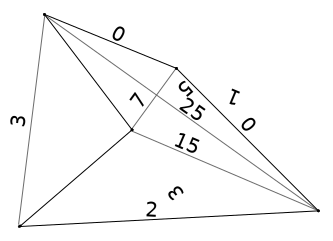
\includegraphics[height=3cm]{complexity/langcomplexity/pictures/tsp}
\end{center}
\begin{example}[Relevance]
	A circuit is basically a round-trip over a board. As such, minimizing 
	the resistance, \dots encompasses solving the TSP.
\end{example}

\paragraph{Satisfiability of boolean expressions (SAT)}
Given a boolean expression with variables, is there a way to assign the 
variables, so that the whole expression is true?
\begin{example}[Relevance]
	When modelling certain domains, for example in a system of artificial
	intelligence, constraints are often expressed as boolean expressions or can
	be converted to them\footnote{See \cite{russell1995artificial}}. Checking
	whether the constraints can be satisfied at all can already solve problems:
	If we have the facts $F$ and the hypothesis $H$, then $H$ fits the facts, if
	and only if $F\wedge\lnot H$ is \emph{not} satisfiable.
\end{example}
\subsubsection{Reductions}
SAT is an extremely handy problem to reduce to, so the following reductions 
will mostly feature that.
\paragraph{SAT reduces to TSP}
\TODO
\paragraph{TSP reduces to SAT}
\TODO
\paragraph{Factorization reduces to TSP}
\TODO

\paragraph{CFG reduces to SAT}
\TODO

\subsection{Hardness and completeness}
We saw that in computability, there seems to be a natural border of 
computability, in which \WHILE, Turing machines and nearly any reasonably 
strong language reside. It was not too surprising then, that these different 
languages could express each other and themselves by means of interpretation and
compilation. Maybe more surprising is, that the complexity classes \PTIME and 
\NPTIME seem to be a similarly natural border.

\begin{defn}
	For a complexity class $C$, a problem $P$ is \emph{hard}, if 
	$\forall c\in C: c \reducesTo P$.

	The problem $P$ is \emph{$C$-complete}, if $P$ is $C$-hard and $P\in C$.
\end{defn}
\begin{example}
	\begin{itemize}
		\item \FOR is \PTIME-hard, but not complete, because not all \FOR programms run in \PTIME.
		\item \TM is \WHILE-complete.
	\end{itemize}
\end{example}
These examples are a bit cheated, since they use extremely large complexity 
classes. But in fact, we have seen two problems already, that are \NPTIME-complete.

\subsubsection{SAT is \NPTIME-complete}
\begin{theorem}
	The satisfiability of boolean formulas is \NPTIME-complete.
\end{theorem}
\begin{proof}
	For completeness, inclusion and universality are required.

	To prove $SAT\in \NPTIME$, we use the guess-and-check definition of 
	\NPTIME. The required certificate in this case is a mapping of the variables to 
	truth-values. This is at most linear in the length of the expression, 
	therefore fulfilling the required \PSPACE length of the certificate. Given the 
	certificate, we can then fully evaluate the expression, which again takes 
	linear time.

	The general idea how to create an $X$-complete problem is to simulate the 
	mode of computation. In the case of space completeness, you fail if you 
	move out of a premarked part of the tape, in the case of 
	\PTIME-completeness, you count down your remaining time and in the case of 
	\NPTIME-completeness, you build a table of possible configurations of the 
	turing machine and see if any of them succeeds\footnote{This proof follows 
	\cite{sipser2006introduction}}.

	% Jones has a more elegant approach, but that requires to introduce the 
	% language SBoole, which then simulates a GOTO program, which simulates a 
	% TM. However the solution is so much prettier, that I consider adapting it 
	% to the known formalisms.
  %
	First assume without loss of generality, that the problem, we want to reduce
	takes at most $n^k$ steps to accept. This means, that we can be in at most 
	\TODO prove rest
\end{proof}
This implies, that SAT can express any other \NPTIME problem with only a 
polynomial slowdown. This also means, that SAT could model any \PTIME 
problem, such as checking context free grammar membership.

On the other hand, we saw that SAT can be reduced to the Traveling Salesman 
Problem, which shows its completeness as well.

There are indeed many relevant problems that are \NPTIME-complete\footnote{So 
many in fact, that the author struggled to find any interesting \PTIME problems}, for 
example maximizing linear functions over linear constraints in the domain of 
integers or optimal scheduling of tasks over multiple processors just to name two.

\subsubsection{\NPTIME and optimization}
\label{np-opti}
While one should keep in mind, that \NPTIME only
describes decision problems, many \NPTIME-complete
problems actually hide an optimization problem. For
example, if we can determine if the traveling
salesman can do the round-trip with cost of at most
$k$, then we can actually find the optimal path:

\begin{algorithmic}[1]
	\State find least $k_0$, so that the round-trip is possible with binary search over $k$
	\For{each edge $e$ in the graph}
		\State Remove the $e$
		\State Check if the round-trip cost increases
		\State If so, reinsert $e$
	\EndFor
\end{algorithmic}

After the algorithm finishes, the only edges in the graph are the ones in the round-trip.

\subsubsection{Help, my problem is \NPTIME-complete}
While being (probably) asymptotically very difficult to solve, 
\NPTIME-complete problems are by no means impossible. There are some 
strategies that can be applied to handle them.
\paragraph{\NPTIME-complete does not necessarily mean slow}
In many cases, the precise algorithm to solve the problem works reasonably 
fast in most cases, but explodes for some abnormal cases. If these abnormal 
cases don't occur in normal input data, the algorithm is still save.

For example, if we are solving SAT, but the inputs take only the form of horn 
clauses (for example $\bigwedge x_i \rightarrow y$), then the problem is 
solvable in \PTIME. 

It could also be, that the algorithm runs in $\mathcal{O}((1+\varepsilon)^n)$ 
for some small $\varepsilon$. Then $n$ would have to be very big for it to be problematic.
\paragraph{Parametrization}
The problem might be slow in general, but there are different parameters to 
the problem, that, when fixed, make the algorithm polynomial. Only increasing 
these parameters then give the full problem. 

For example, checking if a given program in the ML language\footnote{Java or
	C++ would be no better as anyone who ever used template code knows. Actually,
	C++ templates are even Turing-complete \cite{veldhuizen2003c++}}
does not violate any typing (i.e.\ a cast would be necessary) is
\NPTIME-complete\footnote{See \cite{downey1999parameterized}}, but if we
parametrize by the number of type definitions in the system, we have merely a
polynomial runtime.
\paragraph{Approximation}
As seen in section~\ref{np-opti}, many \NPTIME-complete problems are actually
optimization problems in disguise. Instead of looking for \emph{the} optimal
solution, often it is enough to settle for a sub-optimal, but good enough
solution.  In this text, we didn't develop the necessary tools to analyse such
inaccurate algorithms, but such algorithms can come --provably-- very close to
an optimal solution, while taking only polynomial time.

\subsection{Other complexity classes}
The complexity classes introduced are of course only scratching the surface 
of the fascinating topic of complexity theory. There are many different modes 
of computation, that do not factor into \PTIME or \NPTIME, for example 
parallelism, which will be of ever greater importance, as the number of cores 
of computers increase, when the sequencial speed cannot. A bit further down 
the road, the quantum computer will get its share.

\paragraph{$\mathtt{NC}$}
stands for Nick's class\footnote{honoring Nick Pippenger} and
has been described as the class of well-parallelizable 
problems\citationneeded. It is known that $\mathtt{NC} \subset \PTIME$, but it is unknown, 
whether this inclusion is proper. Similarly to \NPTIME-complete problems, 
\PTIME-complete problems, such as CFG, are analyzed to prove this. 

\paragraph{$\mathtt{BQP}$}
is the class of bounded-error polynomial-time quantum computable decision 
problems. Bounded error compensates for the fact that quantum computation is, 
in order to achieve its full strength, random. Bounding the error means that 
it gives the wrong answer at most $0<\varepsilon<\frac{1}{2}$ of the time, where 
$\varepsilon$ is often arbitrarily chosen to be $\frac{1}{3}$. Given a 
procedure in $\mathtt{BQP}$, it is easy to see, that we can lower the 
probability of error arbitrarily low by running the procedure multiple times 
and taking the average answer.

It is possible to simulate a quantum computation in \PSPACE, and it is 
possible to simulate a deterministic computation on a quantum computer, so 
$\PTIME \subset \mathtt{BQP} \subset \PSPACE$, but again, all inclusions are 
suspected, but not proven, to be proper.

The connection to \NPTIME is unknown, but $\NPTIME\subset \mathtt{BQP}$ would 
imply $\NPTIME\neq \PTIME$.

\subsection{Why \PTIME is probably not \NPTIME}
\cite{impagliazzo1995personal}


\bibliography{biblio}{}
\bibliographystyle{plain}

%\begin{appendices}
	%\include*{appendix}
%\end{appendices}
\end{document}
